%==============================================================================
%  Note on delay processing in SuperMoTo
%
%  Why the analysis carries two different delay estimators, what each one
%  actually measures, why they disagree, where each enters the correction, a
%  defect found in the multi-speaker path, and the subwoofer trim that replaced
%  it. Sections 9 and 10 describe code that is now in the software.
%
%  Build:  pdflatex note_on_delay_processing.tex   (twice, for references)
%
%  (c) 2023-2026 Olivier Doare - LGPL-3.0-or-later
%==============================================================================
\documentclass[11pt,a4paper]{article}

\usepackage[utf8]{inputenc}
\usepackage[T1]{fontenc}
\usepackage{lmodern}
\usepackage[margin=2.5cm]{geometry}
\usepackage{amsmath}
\usepackage{amssymb}
\usepackage{booktabs}
\usepackage{tabularx}
\usepackage{enumitem}
\usepackage{xcolor}
\usepackage{tikz}
\usetikzlibrary{positioning,arrows.meta,calc,fit,backgrounds}
\usepackage{pgfplots}
\pgfplotsset{compat=1.17}
\usepackage{siunitx}
\DeclareSIUnit{\dB}{dB}
\usepackage{fancyhdr}

\definecolor{smtblue}{HTML}{2E6DB4}
\definecolor{smtgold}{HTML}{C9A227}
\definecolor{smtgreen}{HTML}{3FA34D}
\definecolor{smtred}{HTML}{B4472E}
\definecolor{smtpanel}{HTML}{2B2F36}

\usepackage[colorlinks=true,linkcolor=smtblue,urlcolor=smtblue]{hyperref}

\pagestyle{fancy}
\fancyhf{}
\fancyhead[L]{\small Note on delay processing}
\fancyhead[R]{\small SuperMoTo}
\fancyfoot[C]{\thepage}
\renewcommand{\headrulewidth}{0.4pt}

% Code references: \srcref{file}{line}. The \discretionary lets TeX break
% between the file name and the line number rather than overrunning the margin.
\newcommand{\srcref}[2]{\texttt{\small #1}\discretionary{}{}{}\texttt{\small :#2}}
\newcommand{\code}[1]{\texttt{\small #1}}

% Typewriter identifiers do not hyphenate; give the line breaker room instead of
% letting them overrun the margin.
\setlength{\emergencystretch}{3em}

% A boxed remark
\newenvironment{remark}[1]
  {\par\medskip\noindent\begin{tabular}{@{}p{0.03\textwidth}p{0.93\textwidth}@{}}
   \textcolor{smtblue}{\rule{2pt}{\baselineskip}} & \textbf{#1}\\[2pt] & \ignorespaces}
  {\end{tabular}\par\medskip}

\title{\bfseries Note on delay processing in SuperMoTo\\
       \large Two estimators, what each measures, and where they enter the correction}
\author{}
\date{September 2026}

\begin{document}
\maketitle
\thispagestyle{fancy}

\begin{abstract}
\noindent
SuperMoTo's analysis carries two independent ways of measuring ``how much later
does this arrive''. One is the peak of the impulse response, used to align
several loudspeakers to one listening position. The other is the slope of the
subwoofer's phase around the crossover, used to integrate a subwoofer with the
mains. They are easily taken for two ways of measuring the same thing. They
are not: they measure different physical quantities, they can
differ by several milliseconds, and each is the wrong tool for the other's job.

This note establishes the conventions used throughout the analysis code, defines
both estimators precisely, derives why they disagree and by how much, shows that
only one of the two is even available for the multi-speaker problem, and derives
the identity that relates the applied output delays to the delay the correction
filter assumes. That identity was violated by the group-analysis code, silently
and only in layouts where the subwoofer is not the most distant driver;
Section~\ref{sec:defect} gives the defect, its magnitude and why it went
unnoticed, and Section~\ref{sec:proposal} documents the fix and the single
subwoofer trim that now exposes the choice between the two estimators to the
user.
\end{abstract}

\tableofcontents

%==============================================================================
\section{Purpose and scope}

The material here covers the delay handling in \code{AnalysisEngine} (the
single-speaker analysis) and \code{SpeakerGroupAnalysis} (the multi-speaker
alignment). It does not cover the magnitude correction, the smoothing, the
microphone calibration or the swept-sine deconvolution except where those
interact with the timing.

Everything stated about the code refers to the state of the repository at commit
\code{2ddca73}. Line references are given as \srcref{file}{line}.

%==============================================================================
\section{Relation to existing work}
\label{sec:litt}

Every ingredient below appears somewhere in the literature. What seems not to be
written down is the combination, and two specific results that fall out of it.
This section says which is which, so the note can be read as an engineering
account of one signal chain rather than as a claim about acoustics.

\subsection{What the literature already covers}

\paragraph{Measurement.} Sweep-based transfer-function measurement, including
the handling of the bulk delay, is standard: M\"uller and Massarani
\cite{Muller2001} is the reference treatment, and Novak \emph{et al.}
\cite{Novak2015} give the synchronized swept sine used by this software. Nothing
in Section~\ref{sec:peakpick} is new; it is recorded here only to fix the
conventions the rest of the note depends on.

\paragraph{Time-delay estimation.} The peak pick of \eqref{eq:peak} is a crude
member of a well-developed family. Knapp and Carter \cite{Knapp1976} derive the
maximum-likelihood estimator and the prefiltering that goes with it, and the
classical result of that literature is that the variance of any delay estimate
scales inversely with the signal's \emph{mean-square bandwidth}, the observation
time and the signal-to-noise ratio. That is the rigorous form of the argument
made informally in Section~\ref{sec:A-failure}: the accuracy floor for a
subwoofer is set by its bandwidth, and no increase in sample rate touches it. It
also explains why the median over positions in \eqref{eq:estA} helps at all:
it is a crude robustification of an estimator whose optimal form is known.

\paragraph{The frequency-dependent origin.} The physical root of
Section~\ref{sec:disagree} is that a loudspeaker has no single point of origin.
Vanderkooy \cite{Vanderkooy2006,Vanderkooy2010} establishes the low-frequency
acoustic centre, shows it generally lies in front of the enclosure, and relates
its position to driver radius, baffle radius and enclosure depth. If the
apparent origin is frequency-dependent, then two estimators interrogating
different bands \emph{must} disagree; the note derives the crossover-filter part
of that disagreement and Vanderkooy covers the radiation part, which is not
treated here at all.

\paragraph{Perceptual weight.} Blauert and Laws \cite{Blauert1978} give the
classical audibility thresholds for group-delay distortion. They bound how much
of the disagreement quantified in Section~\ref{sec:disagree} is worth chasing;
this note quantifies an error without saying when it stops mattering.

\paragraph{Room equalization and spatial averaging.} The multi-position
averaging of Section~\ref{sec:averaging} sits inside a large literature reviewed
by Cecchi, Carini and Spors \cite{Cecchi2018}, which covers prototype responses,
complex versus magnitude averaging and the position-dependence of the result.

\paragraph{Crossover alignment by group delay.} Closest in intent to
Section~\ref{sec:twoproblems} is Kim \cite{Kim2025}, which optimises the
subwoofer--satellite crossover at the listening position by minimising the
maximum absolute group delay in the low band. Like this note, it takes the
position that group delay rather than arrival time is the governing quantity for
sub integration.

\paragraph{Practitioner literature.} The distinction between arrival time and
crossover-region phase is best understood operationally in the sound-reinforcement
literature: McCarthy \cite{McCarthy2016} treats it at length, and van Veen
\cite{vanVeen} publishes a low-frequency acoustic-centre calculator built
directly on Vanderkooy. These sources are not peer-reviewed and do not formalise
the distinction, but the working knowledge is there and predates this note by a
long way.

\subsection{What this note adds}

Three things, all of them properties of a particular processing chain rather
than of acoustics, and none of which I have found stated in the sources above.

\begin{enumerate}[leftmargin=*]
\item \textbf{Estimator B is structurally unavailable for speaker-to-speaker
  alignment} (Section~\ref{sec:twoproblems}). This is not a statement about
  physics but about the order of operations: because per-curve delay removal
  \eqref{eq:removal} precedes coherent spatial averaging \eqref{eq:avg}, the
  relative timing between two speakers is destroyed before any phase could be
  fitted. Any correction scheme that averages coherently across positions
  inherits this constraint, and it explains why the two estimators cannot simply
  be unified: the subwoofer is a special case only because
  \eqref{eq:anchor} deliberately preserves one relationship.

\item \textbf{The alignment identity for a shared subwoofer}
  (Section~\ref{sec:identity}). That the correction must assume the delay it
  will actually be given is obvious for two sources, and implicit throughout the
  practitioner literature. The generalisation to $N$ loudspeakers sharing one
  subwoofer that \emph{also} receives a bulk delay (giving
  $T_i = a_i - a_s$ rather than $T_i = a_i$) appears not to be recorded, and
  the defect of Section~\ref{sec:defect} is exactly what its absence costs.

\item \textbf{A validity condition on the phase-slope estimator}
  \eqref{eq:smoothrot}. Complex smoothing is standard practice and its effect on
  magnitude is well understood; the bound relating smoothing width to the
  largest offset the estimator can still resolve makes explicit when the
  estimate silently stops meaning anything, and is cheap enough to evaluate at
  run time (Section~\ref{sec:proposal}).
\end{enumerate}

None of this is deep. It is written down because each point is the kind of thing
that is obvious once stated and easy to get wrong in code otherwise, as
Section~\ref{sec:defect} demonstrates.

%==============================================================================
\section{Conventions and notation}

\subsection{Sign convention}

The convention is fixed by the code and not by preference, so it is worth
deriving rather than asserting. JUCE's \code{performRealOnlyForwardTransform}
computes
%
\begin{equation}
  X[k] \;=\; \sum_{n=0}^{W-1} x[n]\, e^{-j 2\pi k n / W},
\end{equation}
%
and the Welch estimate at \srcref{AnalysisEngine.cpp}{265} is the standard
$H_1$ form
%
\begin{equation}
  H[k] \;=\; \frac{P_{xy}[k]}{P_{xx}[k]}
        \;=\; \frac{\sum_{\text{seg}} \overline{X[k]}\, Y[k]}
                   {\sum_{\text{seg}} \bigl|X[k]\bigr|^2}\,,
  \label{eq:h1}
\end{equation}
%
with $x$ the sent signal and $y$ the recorded one. If $y[n] = x[n-\delta]$ then
$Y[k] = X[k]\,e^{-j2\pi k \delta/W}$, so
%
\begin{equation}
  \boxed{\;\text{a pure delay } \tau \text{ contributes } e^{-j 2\pi f \tau}\;}
  \label{eq:sign}
\end{equation}
%
This is confirmed by the removal step at \srcref{AnalysisEngine.cpp}{313--317},
which multiplies by $e^{+j 2\pi k \delta / W}$ to cancel it. Bin $k$ corresponds
to $f_k = k f_s / W$, and a delay of $\delta$ samples is $\tau = \delta/f_s$, so
$2\pi k \delta / W = 2\pi f_k \tau$ as required.

Group delay follows from \eqref{eq:sign} with the usual definition
%
\begin{equation}
  \tau_g(f) \;=\; -\frac{1}{2\pi}\,\frac{\mathrm{d}\varphi}{\mathrm{d}f},
  \qquad \varphi(f) = \arg H(f).
  \label{eq:groupdelay}
\end{equation}

\subsection{Notation}

\begin{center}
\begin{tabularx}{\textwidth}{@{}llX@{}}
\toprule
Symbol & Units & Meaning \\
\midrule
$f_s,\;W,\;k$ & --- & sample rate, analysis window length, FFT bin index \\
$p = 1\ldots P$ & --- & microphone position index within one measurement set \\
$H_i^{(p)}(f)$ & --- & raw measured transfer function of entry $i$ at position $p$ \\
$\delta_i^{(p)}$ & samples & peak-picked delay of that measurement \\
$d_i$ & ms & aggregate propagation delay of entry $i$ (median over $p$) \\
$\hat H_i(f)$ & --- & delay-removed spatial average for entry $i$ \\
$S_i(f)$ & --- & sub average \emph{anchored on entry $i$'s} delays \\
$a_i$ & ms & bulk delay physically applied to output $i$ \\
$T_i$ & ms & delay the correction for $i$ \emph{assumes} is applied (\code{timeAlignMs}) \\
$c_i(f)$ & --- & designed correction filter for entry $i$ \\
$f_x$ & Hz & crossover frequency \\
$\tau_{\mathrm{arr}}$ & ms & time-of-arrival estimate (Estimator A) \\
$\tau_{\mathrm{grp}}$ & ms & crossover-band group-delay estimate (Estimator B) \\
\bottomrule
\end{tabularx}
\end{center}

Throughout, the subscript $m$ denotes a main (full-range) loudspeaker and $s$
the subwoofer.

%==============================================================================
\section{From measurement files to spectra}

\subsection{Per-file transfer function}

Each measurement file carries two channels: the stimulus actually sent and the
microphone recording. The transfer function is estimated either by the Welch
$H_1$ estimator \eqref{eq:h1} over 50\,\% overlapping Hann-windowed segments, or,
when the manifest records a synchronized swept sine, by deconvolution with the
sweep's analytic inverse. The distinction does not matter for anything in this
note; both produce a complex $H[k]$ on the same bin grid, with the same sign
convention \eqref{eq:sign}.

\subsection{Delay estimate and removal}
\label{sec:peakpick}

For each file the engine takes the inverse transform of $H$ and picks the sample
of largest absolute value (\srcref{AnalysisEngine.cpp}{283--303}):
%
\begin{align}
  h[n] &= \frac{1}{W}\sum_{k} H[k]\, e^{+j2\pi k n/W}, \qquad n = 0\ldots W-1,\\
  n^\star &= \arg\max_{0 \le n < W} \bigl| h[n] \bigr| .
  \label{eq:peak}
\end{align}
%
The peak index alone is ambiguous, because the inverse transform is periodic:
sample $n$ and sample $n-W$ are the same point on the circle. A measurement
whose recorded channel \emph{leads} the reference (a negative delay, which
arises whenever the sent channel is itself delayed relative to what reached the
converter) therefore does not put its peak near $n = 0$ but near $n = W-1$,
and reading the index literally would report it as a delay of almost a whole
window. The code resolves this by cutting the circle at its halfway point:
%
\begin{equation}
  \delta \;=\;
  \begin{cases}
    n^\star, & n^\star \le W/2,\\[2pt]
    n^\star - W, & n^\star > W/2,
  \end{cases}
  \qquad n^\star = \arg\max_n |h[n]|,
  \label{eq:wrap}
\end{equation}
%
so the representable range is $-W/2 \le \delta \le W/2$, symmetric about zero.

Two consequences follow. The negative half of the range is what makes the
anchoring of Section~\ref{sec:anchor} well behaved: a subwoofer nearer than the
main it is paired with produces a genuinely negative residual, and
\eqref{eq:wrap} represents it rather than wrapping it to a large positive one.
And the positive half sets a ceiling: a true delay beyond $W/2$ is reported as a
negative one, with no indication that it has happened. The window sizes offered
run from $2^{14}$ to $2^{18}$, so the tightest case is $W/2 = 8192$ samples,
about \SI{171}{\milli\second} or \SI{58}{\metre} of path at
$f_s = \SI{48}{\kilo\hertz}$. No room measurement approaches that, so the
ceiling is not a practical limit here. But it is unconditional, and because
\eqref{eq:groupdelays} takes a maximum over entries and then differences, a
single wrapped entry would corrupt the whole group's alignment rather than just
its own.

The linear phase is then divided out,
%
\begin{equation}
  \hat H^{(p)}[k] \;=\; H^{(p)}[k]\; e^{+j 2\pi k \delta^{(p)} / W},
  \label{eq:removal}
\end{equation}
%
leaving a curve whose phase is zero-referenced to its own arrival.

\subsection{Spatial averaging, and why removal must come first}
\label{sec:averaging}

The set for one loudspeaker is averaged \emph{coherently} across positions
(\srcref{AnalysisEngine.cpp}{392}):
%
\begin{equation}
  \hat H_i(f) \;=\; \frac{1}{P}\sum_{p=1}^{P} \hat H_i^{(p)}(f).
  \label{eq:avg}
\end{equation}
%
Removal \eqref{eq:removal} is what makes this possible. Without it, positions
differing by even a few centimetres would carry phase differences approaching
$\pi$ at a few kilohertz and the vector sum would collapse.

\begin{remark}{Consequence}
Equation~\eqref{eq:avg} destroys absolute timing. After averaging, the only
surviving record of when anything arrived is the set of scalars
$\{\delta_i^{(p)}\}$, i.e.\ $d_i$. This single fact is the reason the two
estimators cannot be interchanged, and is developed in
Section~\ref{sec:twoproblems}.
\end{remark}

\subsection{The subwoofer anchoring}
\label{sec:anchor}

The subwoofer set is treated differently. When it is loaded into a main
speaker's engine, each sub measurement is \emph{not} given its own peak-picked
delay; it is forced to the delay of the main measurement taken at the same
microphone position (\srcref{AnalysisEngine.cpp}{125--131}):
%
\begin{equation}
  S_i^{(p)}[k] \;=\; H_s^{(p)}[k]\; e^{+j 2\pi k \delta_{i}^{(p)} / W},
  \qquad
  S_i(f) = \frac{1}{P}\sum_p S_i^{(p)}(f).
  \label{eq:anchor}
\end{equation}
%
Because the main's delay, not the sub's, is removed, $S_i$ retains the
main-to-sub timing difference as a residual linear phase. This residual is the
entire basis of Estimator B, so it is written out here exactly rather than left
to inspection.

Separate each raw sub measurement into its propagation delay and everything
else,
%
\begin{equation}
  H_s^{(p)}(f) \;=\; \Lambda_s^{(p)}(f)\; e^{-j 2\pi f d_s^{(p)}},
  \label{eq:lambda}
\end{equation}
%
where $\Lambda_s^{(p)}$ is the subwoofer's \emph{intrinsic} response at that
position: driver, enclosure, low-pass filter, and whatever the room adds. The
symbol is deliberately not $G$, which in acoustics is reserved for a Green's
function; $\Lambda_s$ is not a Green's function but a measured transfer
function with the bulk propagation term factored out. Substituting into
\eqref{eq:anchor} and writing the per-position residual delay as a mean plus a
deviation,
%
\begin{equation}
  d_s^{(p)} - d_i^{(p)} \;=\; \Delta_{si} + \epsilon^{(p)},
  \qquad \textstyle\sum_p \epsilon^{(p)} = 0,
\end{equation}
%
gives the exact expression
%
\begin{equation}
  S_i(f) \;=\; e^{-j 2\pi f \Delta_{si}}\;
               \underbrace{\frac{1}{P}\sum_{p=1}^{P}
                 \Lambda_s^{(p)}(f)\, e^{-j 2\pi f \epsilon^{(p)}}}_{\textstyle \equiv\, \bar\Lambda_s(f)} .
  \label{eq:sub-exact}
\end{equation}
%
So the clean form
%
\begin{equation}
  S_i(f) \;\simeq\; \bar\Lambda_s(f)\; e^{-j 2\pi f (d_s - d_i)}
  \label{eq:sub-structure}
\end{equation}
%
is an approximation on two counts, set out below.
%
\begin{enumerate}[leftmargin=*]
\item \textbf{Aggregation.} $\Delta_{si}$ is the mean of the per-position
  residuals, whereas $d_s$ and $d_i$ as defined in \eqref{eq:estA} are
  \emph{medians} of separately peak-picked delays. The two coincide only when
  the residuals are symmetrically distributed and the peak picks are unbiased.
  Writing $d_s - d_i$ in \eqref{eq:sub-structure} is therefore a first-moment
  substitution, not an identity.
\item \textbf{Separability.} The bracket in \eqref{eq:sub-exact} is not a
  position-independent function times a common phasor: $\Lambda_s^{(p)}$ itself
  varies with position (room modes below \SI{100}{\hertz} are strongly
  position-dependent), and it is weighted by $e^{-j2\pi f \epsilon^{(p)}}$. Only
  when $2\pi f |\epsilon^{(p)}| \ll 1$ across the band of interest does
  $\bar\Lambda_s$ behave like a single intrinsic response.
\end{enumerate}
%
The second condition is the quantitative form of the spatial-spread caveat in
Section~\ref{sec:B-failure}: it fails from above, at the top of the fit band,
and it fails silently.

%==============================================================================
\section{Estimator A: time of arrival}
\label{sec:A}

\subsection{Definition}

The aggregate propagation delay of an entry is the median of its per-file
peak positions (\srcref{AnalysisEngine.cpp}{73}):
%
\begin{equation}
  \boxed{\;
  d_i \;=\; \frac{1000}{f_s}\;\operatorname{median}_{p}\;\delta_i^{(p)}
  \quad [\mathrm{ms}]\;}
  \label{eq:estA}
\end{equation}
%
The median rather than the mean is deliberate: one microphone position that
latches onto a reflection or a mode does not move the result.

This estimator is computed on the \emph{raw} $H$, before smoothing and before
the microphone calibration is applied. Both of those are magnitude-dominated
operations and neither would improve a peak pick.

\subsection{Resolution}

The peak search \eqref{eq:peak} is on the integer sample grid, so the
quantisation is
%
\begin{equation}
  \Delta \tau = \frac{1}{f_s} = \SI{20.8}{\micro\second}
  \quad\text{at } f_s = \SI{48}{\kilo\hertz},
\end{equation}
%
about \SI{7}{\milli\metre} of path. That is far finer than needed, and it is
never the limiting factor. The limit is the width of the impulse itself.

\subsection{Failure modes}
\label{sec:A-failure}

\begin{enumerate}[leftmargin=*]
\item \textbf{Band limitation.} A signal band-limited to $f_{\max}$ has an
  impulse response no narrower than a sinc of first null $1/(2 f_{\max})$, i.e.\
  a main lobe of width
  %
  \begin{equation}
    \Delta t \;\simeq\; \frac{1}{f_{\max}}.
    \label{eq:lobe}
  \end{equation}
  %
  For a full-range loudspeaker measured to \SI{20}{\kilo\hertz} this is
  \SI{50}{\micro\second} and the peak is unambiguous. For a subwoofer passing
  nothing above \SI{100}{\hertz} it is \SI{10}{\milli\second}. Picking the
  largest sample of a lobe \SI{10}{\milli\second} wide is a millisecond-scale
  estimate at best, whatever the sample rate.

\item \textbf{Room modes.} Below \SI{100}{\hertz} a modal decay can be
  comparable in amplitude to the direct arrival and arbitrarily placed in time.
  The peak may not be the direct sound at all.

\item \textbf{Minimum-phase group delay.} A loudspeaker's own high-pass
  alignment and any crossover filtering shift and skew the lobe. What
  \eqref{eq:peak} returns is neither the onset nor the group delay but something
  in between, and the relationship is not fixed. Section~\ref{sec:disagree}
  develops this.
\end{enumerate}

\begin{remark}{Summary}
Estimator A is excellent for a full-range source and progressively meaningless
as the source's bandwidth shrinks. For a subwoofer it is the weakest tool
available.
\end{remark}

%==============================================================================
\section{Estimator B: crossover-band group delay}
\label{sec:B}

\subsection{Definition}

Taking the anchored sub average $S_i$ of \eqref{eq:anchor} and its phase
$\varphi_S(f) = \arg S_i(f)$, the engine samples $N = 48$ points spaced
logarithmically over one octave either side of the crossover,
%
\begin{equation}
  f_n \;=\; f_{\mathrm{lo}} \left(\frac{f_{\mathrm{hi}}}{f_{\mathrm{lo}}}\right)^{\!\!n/(N-1)},
  \qquad
  f_{\mathrm{lo}} = \tfrac{1}{2} f_x, \quad f_{\mathrm{hi}} = 2 f_x,
\end{equation}
%
unwraps the phase by forcing successive differences into $(-\pi, \pi]$, and takes
the least-squares slope weighted by the measured power
$w_n = |S_i(f_n)|^2$ (\srcref{AnalysisEngine.cpp}{569--620}):
%
\begin{equation}
  \sigma \;=\;
  \frac{\sum_n w_n (f_n - \bar f)(\tilde\varphi_n - \bar\varphi)}
       {\sum_n w_n (f_n - \bar f)^2},
  \qquad
  \bar f = \frac{\sum w_n f_n}{\sum w_n}, \quad
  \bar\varphi = \frac{\sum w_n \tilde\varphi_n}{\sum w_n},
  \qquad
  \boxed{\;\tau_{\mathrm{grp}} \;=\; -\frac{\sigma}{2\pi}\;}
  \label{eq:estB}
\end{equation}
%
The weighting is not a refinement. Section~\ref{sec:B-failure} shows the
unweighted fit is unusable in exactly the band this estimator is built for.
%
with $\tilde\varphi$ the unwrapped phase, clamped to $\pm\SI{40}{\milli\second}$
on return. The minus sign is bookkeeping: by \eqref{eq:sign} a lagging source
has a phase that \emph{decreases} with frequency, so the fitted slope $\sigma$
is negative for a subwoofer that arrives late, and the minus makes
$\tau_{\mathrm{grp}}$ come out positive in that case.

What the sign does not tell you is the more important point, and it is easy to
read \eqref{eq:estB} as though it did. A least-squares slope over a band returns
the \emph{average group delay across that band}. That number coincides with an
arrival time only if the phase is exactly linear over the band, that is, only
if the source behaves as a pure delay there. A subwoofer near its crossover is
precisely the case where it does not: Figure~\ref{fig:lr4} shows the group delay
varying by some 20\,\% across the fit band for a textbook filter alone, before
the driver, the enclosure and the room contribute. So $\tau_{\mathrm{grp}}$ is a
summary statistic of a frequency-dependent quantity, chosen because the
crossover region is where the summation happens. It is not the time at which
anything arrives, and Estimator A is not a coarse measurement of it.

\subsection{What it actually measures}

Substituting \eqref{eq:sub-structure} into \eqref{eq:estB},
%
\begin{equation}
  \tau_{\mathrm{grp}}
  \;=\; \underbrace{(d_s - d_m)}_{\text{path difference}}
  \;+\; \underbrace{\Bigl\langle -\tfrac{1}{2\pi}\tfrac{\mathrm{d}}{\mathrm{d}f}\arg \bar\Lambda_s(f) \Bigr\rangle_{[f_x/2,\,2f_x]}}_{\text{sub's own group delay in the band}},
  \label{eq:B-decomp}
\end{equation}
%
where $\langle\cdot\rangle$ denotes the least-squares band average. Estimator B
therefore reports the \emph{total} effective lateness of the subwoofer's energy
in the crossover region, geometry and filtering together. That is precisely the
quantity that governs whether the two sources add or cancel there.

\subsection{Unwrapping is not a limitation}

The obvious worry is aliasing of the unwrap. It does not bite here. The
logarithmic spacing gives a ratio $f_{n+1}/f_n = 4^{1/47} \approx 1.0299$, so at
the top of the band ($f_x = \SI{80}{\hertz}$, $f_{\mathrm{hi}} =
\SI{160}{\hertz}$) the largest step is $\Delta f \approx \SI{4.7}{\hertz}$.
Correct unwrapping requires $|\Delta\varphi| < \pi$ between samples, i.e.
%
\begin{equation}
  \tau \;<\; \frac{1}{2\,\Delta f} \;\approx\; \SI{107}{\milli\second},
\end{equation}
%
comfortably beyond the $\pm\SI{40}{\milli\second}$ the result is clamped to.

\subsection{Failure modes}
\label{sec:B-failure}

\begin{enumerate}[leftmargin=*]
\item \textbf{The fit band reaches into the stopband.} This is the dominant
  failure and the reason \eqref{eq:estB} is weighted. The band
  $[f_x/2,\,2f_x]$ is chosen around the crossover, but a subwoofer is already
  far down at its top: on a real five-position measurement crossed at
  \SI{85}{\hertz}, $|S|$ falls from \SI{-6}{\dB} at \SI{60}{\hertz} to
  \SI{-18}{\dB} at \SI{120}{\hertz} and \SI{-50}{\dB} at \SI{170}{\hertz}, a
  spread of \SI{46}{\dB} across the fit band, and the position-to-position
  coherence collapses from $0.99$ to $0.60$ over the same span. An unweighted
  fit gives that noise the same say as the passband, and the estimate then
  walks with the crossover setting:
  %
  \begin{center}
  \begin{tabular}{@{}lccccc@{}}
  \toprule
  $f_x$ (Hz) & 60 & 85 & 100 & 120 & 150\\
  \midrule
  $\tau_{\mathrm{grp}}$, unweighted (ms) & 27.6 & 21.8 & 17.7 & 13.7 & 11.3\\
  $\tau_{\mathrm{grp}}$, weighted (ms)   & 26.4 & 31.3 & 32.3 & 34.8 & 30.7\\
  \bottomrule
  \end{tabular}
  \end{center}
  %
  The weighted figure is stable and agrees with the arrival-time estimate for
  the same set (\SI{30.6}{\milli\second}); the unweighted one manufactures a
  disagreement of \SI{8.8}{\milli\second} at \SI{85}{\hertz} that is pure
  artefact of fitting through noise. Acting on it moves the alignment
  \SI{9}{\milli\second} away from correct.

\item \textbf{Smoothing dependence.} Estimator B runs on
  \code{subAverageSmoothed}, i.e.\ after complex variable-octave smoothing. A
  smoothing window of relative width $\beta$ (in octaves) at frequency $f$ spans
  $\Delta f \approx \beta f \ln 2$. Across it, a residual delay $\tau$ rotates
  the phasor by
  %
  \begin{equation}
    \Delta\varphi \;\approx\; 2\pi\,\tau\,\beta f \ln 2 .
    \label{eq:smoothrot}
  \end{equation}
  %
  Complex averaging over a rotation approaching $\pi$ collapses the vector sum
  and the phase becomes unreliable. At $f = \SI{160}{\hertz}$ with
  $\beta = 1$ octave, \eqref{eq:smoothrot} reaches $\pi$ at
  $\tau \approx \SI{4.5}{\milli\second}$, entirely within the range of
  offsets one is trying to measure. \emph{Heavy smoothing and a large offset
  together make Estimator B untrustworthy}, and the failure is silent.

\item \textbf{Crossover dependence.} The fit band is $[f_x/2,\, 2f_x]$. Changing
  the crossover control changes the reported offset, because $\bar\Lambda_s$ is not
  minimum-delay-flat: a genuinely frequency-dependent group delay is being
  reduced to one number over a band the user chooses.

\item \textbf{Spatial spread.} By \eqref{eq:anchor}, $S_i$ averages terms whose
  residual delays $d_s^{(p)} - d_i^{(p)}$ differ across positions. A spread of
  $\pm\Delta$ about the mean attenuates the average by roughly
  $\operatorname{sinc}(2 f \Delta)$ and, if the spread is asymmetric, biases the
  slope. For a microphone array spanning a listening area with the sub well off
  the mains' axis, $\Delta$ of \SI{1}{\milli\second} or more is normal.

\item \textbf{Availability.} Estimator B requires a sub set loaded into that
  speaker's engine. It returns $0$ when \code{subAverageSmoothed} is empty.
\end{enumerate}

%==============================================================================
\section{Why the two disagree}
\label{sec:disagree}

\subsection{A minimum-phase filter carries group delay}

The dominant term in \eqref{eq:B-decomp} beyond geometry is the crossover
filter. Take the common case of a fourth-order Linkwitz--Riley low-pass, which
is two cascaded second-order Butterworth sections. With $\Omega = f/f_x$ and
$\omega_x = 2\pi f_x$, one Butterworth section has
%
\begin{equation}
  H_{\mathrm{B2}}(j\Omega) = \frac{1}{1 - \Omega^2 + j\sqrt{2}\,\Omega},
  \qquad
  \varphi = -\arctan\!\frac{\sqrt{2}\,\Omega}{1-\Omega^2},
\end{equation}
%
and differentiating (Appendix~\ref{app:lr4}) gives a closed form. Cascading two:
%
\begin{equation}
  \boxed{\;
  \tau_{\mathrm{LR4}}(\Omega)
  \;=\; \frac{2\sqrt{2}}{\omega_x}\,\frac{1+\Omega^2}{1+\Omega^4}\;}
  \label{eq:lr4}
\end{equation}
%
At both $\Omega = 0$ and $\Omega = 1$ this equals $2\sqrt{2}/\omega_x$, with a
gentle maximum about 20\,\% higher near $\Omega \approx 0.7$. Numerically, for
$f_x = \SI{80}{\hertz}$,
%
\begin{equation}
  \tau_{\mathrm{LR4}} \;=\; \frac{2\sqrt{2}}{2\pi \cdot 80}
  \;=\; \SI{5.63}{\milli\second},
\end{equation}
%
equivalent to about \SI{1.9}{\metre} of apparent extra path, from the filter
alone, with the subwoofer physically where it is.

\begin{figure}[ht]
\centering
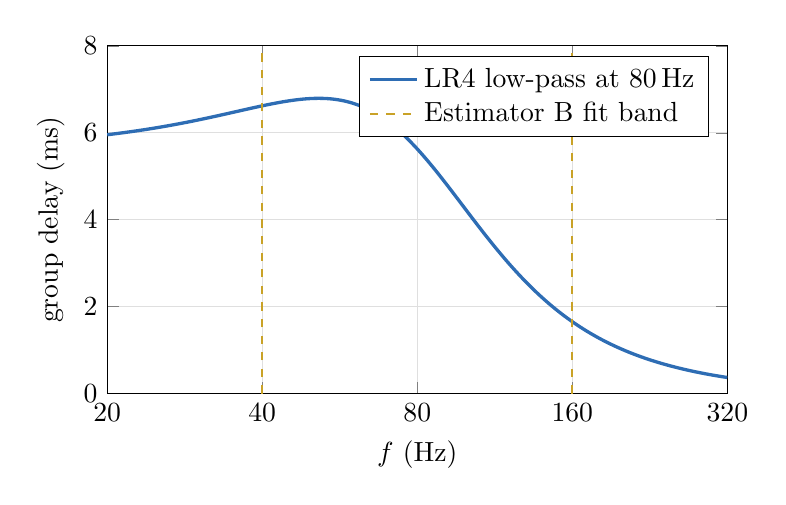
\begin{tikzpicture}
\begin{axis}[
  width=0.78\textwidth, height=6cm,
  xlabel={$f$ (Hz)}, ylabel={group delay (ms)},
  xmode=log, xmin=20, xmax=320,
  ymin=0, ymax=8,
  grid=both, grid style={gray!25},
  legend pos=north east, legend cell align=left,
  xtick={20,40,80,160,320}, xticklabels={20,40,80,160,320},
]
% tau = 2*sqrt(2)/(2*pi*80) * (1+O^2)/(1+O^4) * 1000 ms, O = x/80
\addplot[smtblue, very thick, domain=20:320, samples=200]
  {1000*2*sqrt(2)/(2*pi*80) * (1+(x/80)^2)/(1+(x/80)^4)};
\addlegendentry{LR4 low-pass at \SI{80}{\hertz}}
% the fit band
\addplot[smtgold, dashed, thick] coordinates {(40,0) (40,8)};
\addplot[smtgold, dashed, thick] coordinates {(160,0) (160,8)};
\addlegendentry{Estimator B fit band}
\end{axis}
\end{tikzpicture}
\caption{Group delay of a fourth-order Linkwitz--Riley low-pass at
\SI{80}{\hertz}, equation~\eqref{eq:lr4}, with the band over which Estimator B
fits its slope. The band average is close to \SI{5}{\milli\second}. Estimator A,
picking the peak of a broadband impulse, does not report this figure.}
\label{fig:lr4}
\end{figure}

\subsection{The two estimates, side by side}

Collecting \eqref{eq:estA} and \eqref{eq:B-decomp}, and writing $d$ for what
Estimator A returns for each entry:
%
\begin{align}
  \text{A gives} \quad & d_s - d_m
    \;=\; (\text{path difference}) + (\text{peak shift caused by } \bar\Lambda_s)
    \label{eq:A-content}\\[2pt]
  \text{B gives} \quad & \tau_{\mathrm{grp}}
    \;=\; (\text{path difference}) + \bigl\langle \tau_g[\bar\Lambda_s] \bigr\rangle_{[f_x/2,\,2f_x]}
    \label{eq:B-content}
\end{align}
%
The first terms are the same. The second terms are \emph{not} the same
functional of $\bar\Lambda_s$: one is where a band-limited lobe peaks, the other is the
average slope of the phase over a chosen octave-wide band. There is no general
relation between them.

\begin{remark}{The difference is diagnostic}
The gap $\tau_{\mathrm{grp}} - (d_s - d_m)$ is therefore, to first order, the
part of the subwoofer's lateness that comes from its own filtering rather than
from where it stands. Close to zero means the sub behaves like a delayed copy of
the main and the offset is pure geometry: move the box and the number moves
with it. Several milliseconds means the offset is dominated by the crossover and
driver alignment, and moving the box will not fix it. This is information the
user currently never sees.
\end{remark}

%==============================================================================
\section{Two different alignment problems}
\label{sec:twoproblems}

\subsection{Speaker to speaker: only Estimator A exists}

Consider aligning speakers $i$ and $j$, both full-range, measured at the same
positions. Their engines have independently applied \eqref{eq:removal} with
their own $\delta_i^{(p)}$ and $\delta_j^{(p)}$. Therefore
%
\begin{equation}
  \arg \hat H_i(f) \;\text{ and }\; \arg \hat H_j(f)
  \quad\text{carry no information about } d_i - d_j,
\end{equation}
%
because that difference was divided out, per position, before averaging. The
smoothed averages simply do not contain it. There is no phase slope to fit.

\begin{remark}{Structural conclusion}
Estimator B is not merely a poor choice for speaker-to-speaker alignment; it is
unavailable. It exists only for the main/sub pair, and only because
\eqref{eq:anchor} deliberately preserves that one relationship. Making it
available for an arbitrary pair would require anchoring speaker $j$'s curves on
speaker $i$'s per-position delays, one such average per ordered pair.
\end{remark}

Fortunately Estimator A is the right answer for this problem anyway. Two
full-range sources have essentially the same $G$, so the second terms of
\eqref{eq:A-content} cancel in the difference and the peak pick returns the path
difference cleanly, which is what one wants to equalise so that
transients arrive together.

\subsection{Main to sub: Estimator B is the correct quantity}

Here the two sources have different passbands, and the second terms do not
cancel. Section~\ref{sec:A-failure} showed the sub's peak pick is
millisecond-uncertain in principle; Section~\ref{sec:disagree} showed the filter
contributes several milliseconds that the peak pick does not report in the way
the crossover experiences it. What determines summation at $f_x$ is group delay
at $f_x$. Estimator B measures that directly.

\begin{center}
\begin{tabularx}{\textwidth}{@{}lXX@{}}
\toprule
& \textbf{speaker $\leftrightarrow$ speaker} & \textbf{main $\leftrightarrow$ sub} \\
\midrule
Estimator A & correct and robust & available but weak \\
Estimator B & \emph{not available} (phase destroyed by \eqref{eq:removal}) & correct quantity \\
\midrule
Goal & transients arrive together & sources sum coherently at $f_x$ \\
\bottomrule
\end{tabularx}
\end{center}

%==============================================================================
\section{Where the delays enter the correction}
\label{sec:chain}

\subsection{The signal chain}

\begin{figure}[ht]
\centering
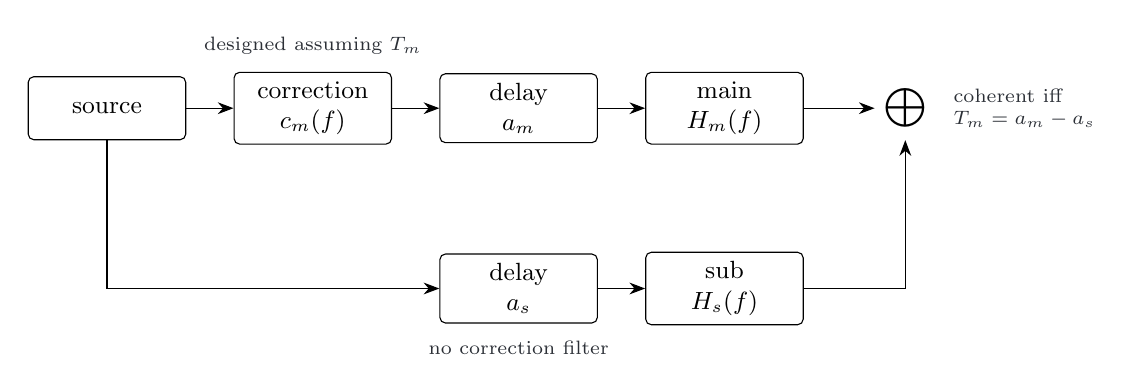
\begin{tikzpicture}[
  node distance=6mm,
  blk/.style={draw, rounded corners=2pt, minimum height=8mm, minimum width=20mm,
              align=center, font=\small, fill=white},
  lbl/.style={font=\scriptsize, text=smtpanel},
  >={Stealth[length=2mm]}
]
\node[blk] (src) {source};
\node[blk, right=of src] (corr) {correction\\$c_m(f)$};
\node[blk, right=of corr] (dm)  {delay\\$a_m$};
\node[blk, right=of dm]  (spk)  {main\\$H_m(f)$};
\node[right=9mm of spk] (sum) {$\displaystyle\bigoplus$};

\node[blk, below=14mm of dm] (ds) {delay\\$a_s$};
\node[blk, right=of ds] (sub) {sub\\$H_s(f)$};

\draw[->] (src) -- (corr);
\draw[->] (corr) -- (dm);
\draw[->] (dm) -- (spk);
\draw[->] (spk) -- (sum);
\draw[->] (src.south) |- (ds);
\draw[->] (ds) -- (sub);
\draw[->] (sub.east) -| (sum);

\node[lbl, above=1mm of corr] {designed assuming $T_m$};
\node[lbl, below=1mm of ds] {no correction filter};
\node[lbl, right=1mm of sum, align=left] {coherent iff\\ $T_m = a_m - a_s$};
\end{tikzpicture}
\caption{Where each delay acts. The correction filter is designed off-line
against an \emph{assumption} $T_m$ about the bulk delays that will be applied;
the alignment identity \eqref{eq:identity} is the condition for that assumption
to be true.}
\label{fig:chain}
\end{figure}

\subsection{How the correction uses $T$}

At \srcref{AnalysisEngine.cpp}{708--716} the designed correction is multiplied,
in the crossover region, by an all-pass built from the sub's unit phasor after
advancing it by $T$:
%
\begin{equation}
  S'(f) \;=\; S_m(f)\; e^{+j 2\pi f T},
  \qquad
  A(f) \;=\; \frac{(1-w) + w\,S'/|S'|}{\bigl|(1-w) + w\,S'/|S'|\bigr|},
  \qquad
  c_m \leftarrow c_m \cdot A,
  \label{eq:allpass}
\end{equation}
%
with $w = w(f)$ the alignment weight, unity at and below $f_x$ and released to
zero one octave above (\srcref{AnalysisEngine.cpp}{610}). Where $w = 1$ the
corrected main's phase is steered onto $\arg S'$. Note that $A$ is renormalised
to $|A| = 1$: the all-pass moves phase and nothing else, which matters in
Section~\ref{sec:phasetype}.

\subsection{The alignment identity}
\label{sec:identity}

Write the raw measured responses in terms of the engine's delay-removed
quantities. From \eqref{eq:removal} and \eqref{eq:anchor},
%
\begin{equation}
  H_m = \hat H_m\, e^{-j2\pi f d_m},
  \qquad
  H_s = S_m\, e^{-j2\pi f d_m},
\end{equation}
%
both referred to the \emph{same} anchor $d_m$. The two acoustic paths reaching
the listener, including the bulk delays actually applied to the outputs, are
%
\begin{align}
  \text{main:} \quad & \hat H_m(f)\, c_m(f)\; e^{-j2\pi f d_m}\; e^{-j 2\pi f a_m},\\
  \text{sub:}  \quad & S_m(f)\; e^{-j2\pi f d_m}\; e^{-j 2\pi f a_s}.
\end{align}
%
Their ratio, which must have zero phase for coherent summation, is
%
\begin{equation}
  R(f) \;=\; \frac{\hat H_m\, c_m}{S_m}\; e^{-j 2\pi f (a_m - a_s)}.
\end{equation}
%
In the crossover region \eqref{eq:allpass} makes $\hat H_m c_m$ proportional to
$S'/|S'| = S_m e^{+j2\pi f T}/|S_m|$, hence
%
\begin{equation}
  \arg R(f) \;=\; 2\pi f\,T \;-\; 2\pi f\,(a_m - a_s)
             \;=\; 2\pi f\,\bigl[\, T - (a_m - a_s) \,\bigr],
\end{equation}
%
which vanishes for all $f$ if and only if
%
\begin{equation}
  \boxed{\;T_m \;=\; a_m - a_s\;}
  \label{eq:identity}
\end{equation}

\begin{remark}{Reading of \eqref{eq:identity}}
$T$ is not ``the delay applied to this speaker''. It is the delay applied to
this speaker \emph{relative to the subwoofer}. The header at
\srcref{AnalysisEngine.h}{145--149} says so in words, ``positive $=$ main is
delayed \dots\ negative $=$ the sub is delayed instead'': a single signed
number encoding a difference.
\end{remark}

\subsection{Where that phase goes: linear versus minimum phase}
\label{sec:phasetype}

Everything above concerns the complex correction $c_i(f)$. What is exported is an
impulse response, and the Phase type control decides how one is made from the
other (\srcref{AnalysisEngine.cpp}{924--1024}). The two paths do not treat the
all-pass \eqref{eq:allpass} alike, and the difference is total rather than one of
degree.

\paragraph{Linear phase.} The full complex spectrum is used, with a half-length
shift to make the (mixed-phase) result causal:
%
\begin{equation}
  h[n] \;=\; \frac{1}{N}\sum_{k=0}^{N-1} c_i(f_k)\, e^{-j\pi k}\, e^{+j 2\pi k n/N},
  \qquad f_k = \tfrac{k}{N} f_s .
  \label{eq:renderlin}
\end{equation}
%
The factor $e^{-j\pi k} = (-1)^k$ is a delay of exactly $N/2$ samples, which is
where the mode's latency comes from. The phase of $c_i$, all-pass included,
survives intact.

\paragraph{Minimum phase.} The impulse is rebuilt from the target
\emph{magnitude} alone by the real-cepstrum method: with
$m(f_k) = \log|c_i(f_k)|$ and $\hat m = \mathcal{F}^{-1}\{m\}$, the anti-causal
half of the cepstrum is folded onto the causal half,
%
\begin{equation}
  w[n] = \begin{cases} 1, & n = 0 \text{ or } n = N/2,\\ 2, & 1 \le n < N/2,\\ 0, & \text{otherwise,}\end{cases}
  \qquad
  c_i^{\min} = \exp\bigl(\mathcal{F}\{w\,\hat m\}\bigr),
  \qquad
  h = \mathcal{F}^{-1}\{c_i^{\min}\}.
  \label{eq:rendermin}
\end{equation}
%
Only $|c_i|$ enters \eqref{eq:rendermin}. And the all-pass is renormalised to
unit magnitude in \eqref{eq:allpass}, $A \leftarrow A/|A|$, precisely so that it
changes no level. Therefore $|c_i|$ does not depend on $T$ at all, and
%
\begin{equation}
  \boxed{\;\frac{\partial h}{\partial T} \;=\; 0 \quad\text{in minimum-phase mode.}\;}
  \label{eq:minphase-null}
\end{equation}

\begin{remark}{Scope of the alignment identity}
Equation~\eqref{eq:identity} therefore has force only in linear-phase mode. Under
minimum phase the subwoofer trim, the crossover frequency and the Invert sub
switch have exactly no effect on the exported FIR: not a reduced effect, none.
What still happens is the bulk time alignment, since $a_i$ and $a_s$ are written
to the outputs as plain delays \eqref{eq:groupdelays} and never pass through the
FIR at all. So the group is still time-aligned on arrival times; it is only the
residual phase steering through the crossover that is absent.

The practical consequence is that the Phase type control is not the
magnitude-versus-phase trade-off its name suggests. It is also a
subwoofer-integration on/off switch, and nothing in the delay machinery of this
section applies while it is set to minimum.
\end{remark}

\paragraph{What the plots show.} The phase read-outs go through
\code{effectiveCorrection()} rather than \code{correction}, so they display
$\arg c_i^{\min}$ from \eqref{eq:rendermin} whenever that is the mode
(\srcref{AnalysisEngine.cpp}{903--921}). Until this was noticed they read
$\arg c_i$ unconditionally and therefore drew, in minimum-phase mode, a phase
correction that would never be exported: the plot did not move at all when the
Phase type was changed. The reconstruction is evaluated on the correction's own
bin grid rather than the FIR's, so the curve is the ideal minimum-phase
equivalent of the designed magnitude and does not model the truncation to
\code{firLength} (which the plot has never modelled in either mode). The
magnitude curves are unaffected, since \eqref{eq:rendermin} preserves $|c_i|$
exactly.

\paragraph{Which subwoofer curve is drawn.} A second frame-of-reference error
sat next to the first. The correction is steered onto $S'$, the sub
\emph{after} the assumed bulk delay \eqref{eq:allpass}, but
\code{getSubPhaseDeg} plotted the raw anchored average $S$, and neither the
Invert sub switch nor the delay moved it. The two curves on the plot were
therefore in different time references, and the feedback they gave was exactly
inverted: with $T$ correctly set the corrected main comes out nearly flat while
the drawn sub still swept through its full offset, so a correct alignment looked
like a gross mismatch; with $T = 0$, before Compute alignment has been pressed,
both curves are steep and lie on top of each other, so doing nothing looked
right. On the measurement of Section~\ref{sec:B-failure}, over the
\SIrange{60}{120}{\hertz} span where that subwoofer has output, the drawn curve
swept \SI{662}{\degree} (nearly two turns) where the curve the correction
actually targets sweeps \SI{89}{\degree}. \code{getSubPhaseDeg} now returns
$\arg S'$, so the corrected main and the subwoofer can be read against each
other, which is the one comparison the plot exists to support.

The effective-correction spectrum is built eagerly, by the two writers
\code{recomputeCorrection()} and \code{setPhaseType()}, never on first use. That keeps every accessor on the class
a pure read once the analysis is done, which the threading contract relies on:
the report figures call these same read-outs from a background export job while
the message thread may be plotting the same engine, and concurrent reads are
safe where a lazily filled cache would not be.

\subsection{The single-speaker panel satisfies it}

In the Analysis pane the user sets $T$ directly with the Mains-delay slider and
the subwoofer output receives no delay from the analysis, so $a_s = 0$ and
\eqref{eq:identity} reduces to $T = a_m$, which is what the slider means. The
recommendation displayed beside it is $\tau_{\mathrm{grp}}$ from
\eqref{eq:estB}. That path is consistent.

%==============================================================================
\section{A defect in the group alignment}
\label{sec:defect}

This section describes the code as it stood at the time of the analysis. It has
since been corrected; Section~\ref{sec:proposal} documents what replaced it. The
derivation is kept because the defect is instructive: it was invisible in the
common case, and masked by an artefact of the very estimator it depended on.

\subsection{Statement}

\code{SpeakerGroupAnalysis::computeAlignment()} derived the applied delays from
Estimator A, referring every entry to the most distant one
(\srcref{SpeakerGroupAnalysis.h}{213--223}):
%
\begin{equation}
  D = \max_{i \in \text{loaded}} d_i,
  \qquad
  a_i = \operatorname{clamp}\bigl(D - d_i,\; 0,\; \SI{100}{\milli\second}\bigr),
  \label{eq:groupdelays}
\end{equation}
%
so the farthest driver gets $a = 0$ and everything else is pushed back to meet
it. The subwoofer, when enabled, participates in \eqref{eq:groupdelays} like any
other entry and receives its own $a_s$, written to its output by
\code{finalizeApply} (\srcref{SpeakerGroupAnalysis.h}{466}).

It then passes, at \srcref{SpeakerGroupAnalysis.h}{229},
%
\begin{equation}
  T_i \;\leftarrow\; a_i,
\end{equation}
%
whereas \eqref{eq:identity} requires $T_i = a_i - a_s$. The error is
%
\begin{equation}
  \boxed{\;\varepsilon \;=\; a_s \;=\; D - d_s\;}
  \label{eq:error}
\end{equation}
%
identical for every speaker in the group, and zero if and only if the subwoofer
is the most distant entry.

\subsection{Worked example}

Front pair at \SI{2}{\metre} ($d = \SI{5.8}{\milli\second}$), surrounds at
\SI{5}{\metre} ($d = \SI{14.6}{\milli\second}$), subwoofer at \SI{3}{\metre}
($d = \SI{8.7}{\milli\second}$, ignoring its filter contribution for clarity).
Then $D = \SI{14.6}{\milli\second}$ and
%
\begin{equation}
  a_s = \SI{5.9}{\milli\second}, \qquad
  a_{\mathrm{front}} = \SI{8.8}{\milli\second}, \qquad
  T_{\mathrm{front}}^{\text{required}} = \SI{2.9}{\milli\second},
\end{equation}
%
but the code passes $T_{\mathrm{front}} = \SI{8.8}{\milli\second}$. The all-pass
\eqref{eq:allpass} is then designed for an offset wrong by
\SI{5.9}{\milli\second}, which at $f_x = \SI{80}{\hertz}$ is
%
\begin{equation}
  \Delta\varphi = 2\pi f_x \varepsilon = 2\pi \cdot 80 \cdot 5.9\times10^{-3}
  \;=\; \SI{2.97}{\radian} \;\approx\; 170^\circ .
\end{equation}
%
The crossover region is steered close to antiphase. The result is worse than
applying no phase alignment at all.

\subsection{Why it has not been noticed}

There are two reasons, and both are instructive.

First, in the ordinary two-channel-plus-sub case the subwoofer usually \emph{is}
the most distant entry, so $a_s = 0$ and \eqref{eq:error} vanishes. Second,
\eqref{eq:B-decomp} shows the sub's measured $d_s$ is inflated by its own filter
group delay (several milliseconds by Figure~\ref{fig:lr4}), which biases it
towards being the maximum. The defect is masked by an artefact of the estimator
it depends on.

It appears when a loudspeaker is genuinely farther than the sub: surrounds in a
large room, a sub near the listening position, or any layout with a wide spread
of distances.

\begin{remark}{Note on the disabled-sub case}
When \code{subEnabled} is false the subwoofer is excluded from
\eqref{eq:groupdelays} and receives no delay, so $a_s = 0$ and passing $T_i =
a_i$ is correct. Speakers' engines may still hold sub data and still apply the
all-pass. The current code is therefore right in that branch and wrong in the
other.
\end{remark}

\subsection{What was changed}

Two edits, both small. The subwoofer's delay is now evaluated \emph{before} the
speaker loop (previously \code{apply(sub)} ran after it, so $a_s$ was not
known at the point it was needed), and the value pushed to each engine is the
difference $a_i - a_s^{\mathrm{eff}}$ rather than $a_i$.
Section~\ref{sec:proposal} gives the result. Equation \eqref{eq:groupdelays} and
the delays written to the outputs are unchanged by the fix itself; only what the
corrections assume about them is.

%==============================================================================
\section{What is implemented}
\label{sec:proposal}

The defect of Section~\ref{sec:defect} is fixed and the subwoofer trim described
below is in the software. This section documents what the code now does; the
alternatives that were rejected on the way are kept at the end, since the reasons
constrain any future change.

\subsection{The alignment identity is now respected}

\code{computeAlignment()} derives the subwoofer's applied delay \emph{before}
the speaker loop and pushes the difference,
%
\begin{equation}
  T_i \;=\; a_i - a_s^{\mathrm{eff}},
  \qquad
  a_s^{\mathrm{eff}} = \begin{cases}
    a_s, & \text{sub loaded and enabled},\\
    0,   & \text{otherwise,}
  \end{cases}
\end{equation}
%
which is \eqref{eq:identity}. When the subwoofer is excluded from the alignment
it receives no delay, so measuring the speakers' offsets against zero is correct
in that branch; that was already true of the previous code and is unchanged.

\subsection{The subwoofer trim}

One signed control, \code{setSubTrimMs()}, offsets the subwoofer against the
whole group. Writing $\Delta$ for its value, the applied delays become
%
\begin{equation}
  a_i = D - d_i + \Sigma, \qquad
  a_s = D - d_s + \Delta + \Sigma,
  \label{eq:trim}
\end{equation}
%
with $D$ the reference of \eqref{eq:groupdelays} and $\Sigma$ a group shift
defined below. Substituting into \eqref{eq:identity},
%
\begin{equation}
  \boxed{\;T_i \;=\; a_i - a_s \;=\; (d_s - d_i) - \Delta\;}
  \label{eq:trim-offset}
\end{equation}
%
The shift cancels, so $\Delta$ moves every speaker's assumed main-to-sub offset
by the same amount, in the opposite sense: a positive trim delays the subwoofer,
which reduces the offset the correction has to make up. One control, one physical
degree of freedom, and \eqref{eq:identity} holds for every value the user can
set.

\paragraph{The group shift.} Only differences are audible, so the whole set is
free to slide in time, and the useful choice is the one with the least latency:
the raw delays are computed first and then shifted so that the \emph{earliest}
entry sits at zero,
%
\begin{equation}
  \Sigma \;=\; -\min_{e \,\in\, \text{loaded}} \bigl(D - d_e + \Delta_e\bigr),
  \qquad \Delta_e = \Delta \text{ for the sub}, \; 0 \text{ otherwise.}
\end{equation}
%
This is what makes a positive trim behave as one expects. Delaying the subwoofer
by \SI{9}{\milli\second} relative to mains already carrying
\SI{30.6}{\milli\second} is realised by \emph{subtracting} it from the mains
($30.6 \to 21.4$, sub at $0$) rather than adding it to the sub (mains at $30.6$,
sub at $9.2$): identical alignment, \SI{9.2}{\milli\second} less latency. A
one-sided shift that only ever adds, which is what the first implementation did,
gives the second, and the extra latency is pure waste. With $\Sigma$ defined this
way $a_e \ge 0$ holds by construction for every entry, so the lower clamp never
fires.

\begin{remark}{Clamps}
Two clamps bound \eqref{eq:trim-offset}, and one of them used to bite in ordinary
use. \code{setTimeAlignMs} originally limited $T$ to
$\pm\SI{40}{\milli\second}$, the range of the single-speaker pane's slider,
carried over without reconsidering it. In a group $T$ is a \emph{difference} of
two delays that each live in $[0, \SI{100}{\milli\second}]$, and on the
measurement discussed in Section~\ref{sec:B-failure}, where
$d_s - d_m = \SI{30.6}{\milli\second}$, it saturated at a trim of only
$\Delta = 30.6 - 40 = \SI{-9.4}{\milli\second}$: the slider kept moving and
nothing further happened. The limit is now $\pm\SI{100}{\milli\second}$, matching
the output delay range.

The upper clamp on $a_e$ at \SI{100}{\milli\second} can still fire on a very
spread group. If it does, \eqref{eq:trim-offset} stops holding for the clamped
entry and its crossover alignment is designed for an offset it will not get.
That corner is still undetected.
\end{remark}

\subsection{The suggested trim}

Estimator B is exposed as a recommendation rather than being applied silently.
Setting $T_i = \tau_{\mathrm{grp},i}$ in \eqref{eq:trim-offset} gives
%
\begin{equation}
  \Delta_i^\star \;=\; (d_s - d_i) - \tau_{\mathrm{grp},i},
  \label{eq:suggest}
\end{equation}
%
which is exactly the disagreement between the two estimators, the quantity
Section~\ref{sec:disagree} identified as diagnostic. Two things follow, and both
are used.

First, by \eqref{eq:A-content} and \eqref{eq:B-content} the geometric term
cancels in \eqref{eq:suggest}, so $\Delta_i^\star$ should be nearly the same for
every speaker: what remains is the subwoofer's own group delay, which does not
depend on which main it is paired with. \code{getSuggestedSubTrimMs()} therefore
returns the \emph{median} over the loaded speakers, and a wide spread across
speakers is itself evidence that one of the two estimates is unreliable.

Second, the sign works out as it should. When the subwoofer's crossover-band
group delay exceeds its arrival-time lateness (the usual case, since its
low-pass contributes several milliseconds that the peak pick does not see),
\eqref{eq:suggest} is negative, so the recommendation is to delay the subwoofer
\emph{less} than pure arrival-time alignment would. That is correct: the filter
has already made it late.

The \code{Use x-over} button writes $\Delta_i^\star$ into the trim. The default
is $\Delta = 0$, i.e. pure arrival-time alignment, which is what the software did
before; the user opts in to the phase-based figure rather than having it imposed.

\subsection{Guard against a silent bad estimate}

Section~\ref{sec:B-failure} showed Estimator B degrading silently under heavy
smoothing, so \eqref{eq:smoothrot} is evaluated and the recommendation withdrawn
when it is not trustworthy. \code{isCrossoverEstimateReliable()} computes the
phasor rotation across the smoothing window at the top of the fit band,
%
\begin{equation}
  \Delta\varphi \;=\; 2\pi\,|\Delta^\star|\,\beta(2 f_x)\,(2 f_x)\,\ln 2 ,
\end{equation}
%
where $\beta(f)$ is the octave fraction \emph{actually in force at $f$}. The two
smoothing controls are anchors at \SI{100}{\hertz} and \SI{10}{\kilo\hertz} and
the fraction between them is log-interpolated, so at \SI{170}{\hertz}
%
\begin{equation}
  \beta \;=\; \beta_{\mathrm{LF}} + 0.115\,(\beta_{\mathrm{HF}} - \beta_{\mathrm{LF}}),
\end{equation}
%
that is \SI{88}{\percent} of the LF setting. Using
$\max(\beta_{\mathrm{LF}}, \beta_{\mathrm{HF}})$ instead, as the first
implementation did, made heavy HF smoothing declare the estimate unusable even
though HF smoothing does essentially nothing at a subwoofer crossover.

The estimate is reported as usable only while $\Delta\varphi < \pi/2$, half the
angle at which the complex average collapses. Past that the \code{Use x-over}
button is disabled and the read-out says why, rather than offering a number that
looks authoritative. The trim itself stays available: the user can always set it
by ear.

\subsection{What the interface shows}

The subwoofer row carries the trim slider (bipolar, $\pm\SI{40}{\milli\second}$,
double-click to zero, matching the Mains-delay slider on the single-speaker
pane), the \code{Use x-over} button, and a read-out of $\Delta^\star$ or of the
reason it is unavailable. Each speaker row keeps its applied delay $a_i$.
Applying the trim re-derives the alignment and re-designs every correction, so it
is coalesced through the same \SI{150}{\milli\second} debounce as the other
shared controls rather than run per drag tick. That coalescing carries an
obligation the first implementation missed: anything that \emph{consumes} the
derived alignment must commit the pending change first. Compute alignment and
Apply \& export now flush the debounce before running, and a tick that arrives
while a background batch owns the engines reschedules itself instead of being
dropped. Without both, a trim set a moment earlier was still sitting in the
slider while the delays written to the outputs were the ones from before it,
which is the same failure mode as Section~\ref{sec:defect} wearing a different
hat: what is applied and what is assumed drift apart. The exported report records the
trim alongside the crossover and the other design settings.

\subsection{Alternatives rejected}

\paragraph{(a) Per-row editable $a_i$.} Rejected. It breaks the invariant of
\eqref{eq:groupdelays} (every entry referred to one reference), so the group
is no longer aligned, and it offers $N$ controls for what is one physical degree
of freedom.

\paragraph{(b) Per-row editable $T_i$, decoupled from $a_i$.} Rejected. It makes
\eqref{eq:identity} violable by the user: the correction would assume a delay
other than the one applied, which is precisely the class of defect described in
Section~\ref{sec:defect}. Reintroducing it as a feature would be perverse.

\paragraph{(c) One subwoofer trim.} Implemented, as above.


%==============================================================================
\section{Summary}

\begin{enumerate}[leftmargin=*]
\item The two estimators measure different physical quantities:
  \eqref{eq:A-content} versus \eqref{eq:B-content}. They share only the
  geometric term.
\item Estimator B is structurally unavailable for speaker-to-speaker alignment,
  because \eqref{eq:removal} destroys the relative phase before averaging. It
  exists for the main/sub pair only because \eqref{eq:anchor} preserves it.
\item Estimator A is correct for speaker-to-speaker and weak for main/sub;
  Estimator B is correct for main/sub. Neither is ``better''.
\item They differ by the sub's own group delay, of order \SI{5}{\milli\second}
  for an LR4 at \SI{80}{\hertz} \eqref{eq:lr4}. That difference is worth showing:
  it separates geometry from filtering.
\item The correction must assume $T_i = a_i - a_s$ \eqref{eq:identity}. The group
  code passed $T_i = a_i$, an error of $a_s$ \eqref{eq:error}, zero only when the
  subwoofer is the most distant entry. This is fixed.
\item The main-to-sub offset is now exposed as a single subwoofer trim
  \eqref{eq:trim}, which keeps the identity true for any value the user sets, and
  whose recommended value \eqref{eq:suggest} is precisely the disagreement
  between the two estimators, withdrawn automatically when the smoothing makes
  it untrustworthy.
\end{enumerate}

%==============================================================================
\appendix
\section{Group delay of the Linkwitz--Riley low-pass}
\label{app:lr4}

For one second-order Butterworth section with $\Omega = f/f_x$,
%
\begin{equation}
  \varphi(\Omega) = -\arctan u, \qquad u = \frac{\sqrt{2}\,\Omega}{1-\Omega^2}.
\end{equation}
%
Then
%
\begin{equation}
  \frac{\mathrm{d}u}{\mathrm{d}\Omega}
  = \frac{\sqrt{2}\,(1+\Omega^2)}{(1-\Omega^2)^2},
  \qquad
  1 + u^2 = \frac{(1-\Omega^2)^2 + 2\Omega^2}{(1-\Omega^2)^2}
          = \frac{1+\Omega^4}{(1-\Omega^2)^2},
\end{equation}
%
so that
%
\begin{equation}
  -\frac{\mathrm{d}\varphi}{\mathrm{d}\Omega}
  = \frac{1}{1+u^2}\,\frac{\mathrm{d}u}{\mathrm{d}\Omega}
  = \frac{\sqrt{2}\,(1+\Omega^2)}{1+\Omega^4}.
\end{equation}
%
With $\tau_g = -\mathrm{d}\varphi/\mathrm{d}\omega =
-(1/\omega_x)\,\mathrm{d}\varphi/\mathrm{d}\Omega$ and two cascaded sections,
equation~\eqref{eq:lr4} follows. Both limits $\Omega \to 0$ and $\Omega = 1$
give $2\sqrt{2}/\omega_x$. The maximum follows from $1 - 2\Omega^2 - \Omega^4 = 0$,
i.e.\ $\Omega = \sqrt{\sqrt{2}-1} \approx 0.644$, where the factor
$(1+\Omega^2)/(1+\Omega^4)$ reaches $1.2071$, about 21\,\% above the value at
DC and at the corner.


%==============================================================================
\begin{thebibliography}{99}

\bibitem{Blauert1978}
J.~Blauert and P.~Laws,
``Group delay distortions in electroacoustical systems'',
\emph{J. Acoust. Soc. Am.} \textbf{63}(5), 1478--1483, 1978.

\bibitem{Cecchi2018}
S.~Cecchi, A.~Carini and S.~Spors,
``Room response equalization --- a review'',
\emph{Applied Sciences} \textbf{8}(1), 16, 2018.
\texttt{doi:10.3390/app8010016}.

\bibitem{Kim2025}
J.~Kim,
``Group delay-driven crossover optimization for subwoofer satellite systems at
listening position'',
\emph{Acta Acustica} \textbf{9}, 51, 2025.
\texttt{doi:10.1051/aacus/2025037}.

\bibitem{Knapp1976}
C.~H.~Knapp and G.~C.~Carter,
``The generalized correlation method for estimation of time delay'',
\emph{IEEE Trans. Acoust., Speech, Signal Process.} \textbf{24}(4), 320--327, 1976.
\texttt{doi:10.1109/TASSP.1976.1162830}.

\bibitem{McCarthy2016}
B.~McCarthy,
\emph{Sound Systems: Design and Optimization}, 3rd ed., Focal Press, 2016.

\bibitem{Muller2001}
S.~M\"uller and P.~Massarani,
``Transfer-function measurement with sweeps'',
\emph{J. Audio Eng. Soc.} \textbf{49}(6), 443--471, 2001.

\bibitem{Novak2015}
A.~Novak, P.~Lotton and L.~Simon,
``Synchronized swept-sine: theory, application, and implementation'',
\emph{J. Audio Eng. Soc.} \textbf{63}(10), 786--798, 2015.

\bibitem{Vanderkooy2006}
J.~Vanderkooy,
``The acoustic center: a new concept for loudspeakers at low frequencies'',
121st AES Convention, San Francisco, paper 6912, 2006.

\bibitem{Vanderkooy2010}
J.~Vanderkooy,
``The low-frequency acoustic center: measurement, theory, and application'',
128th AES Convention, London, paper 7992, 2010.

\bibitem{vanVeen}
M.~van Veen,
``Low-frequency acoustic center calculator'' and related technical notes,
\url{https://www.merlijnvanveen.nl/}.

\end{thebibliography}

\end{document}
